\documentclass[a4paper, 12pt, twoside]{article} 
\usepackage[english]{babel}
\usepackage[utf8]{inputenc}
\usepackage[acronym, toc]{glossaries}
\usepackage{comment}
\usepackage{nomencl}
%\usepackage{minted}
\usepackage{xargs}                      % Use more than one optional parameter in new commands
\usepackage[pdftex, dvipsnames]{xcolor}  % Coloured text etc.
\usepackage[colorinlistoftodos, prependcaption, textsize=tiny]{todonotes}
\usepackage{amsthm}
\usepackage{amssymb}
\usepackage{graphicx}
\usepackage{siunitx}
\usepackage{booktabs}
\graphicspath{{./images/}}

\newcommandx{\unsure}[2][1=]{\todo[linecolor=red, backgroundcolor=red!25, bordercolor=red, #1]{#2}}
\newcommandx{\change}[2][1=]{\todo[linecolor=blue, backgroundcolor=blue!25, bordercolor=blue, #1]{#2}}
\newcommandx{\info}[2][1=]{\todo[linecolor=OliveGreen, backgroundcolor=OliveGreen!25, bordercolor=OliveGreen, #1]{#2}}
\newcommandx{\improvement}[2][1=]{\todo[linecolor=Plum, backgroundcolor=Plum!25, bordercolor=Plum, #1]{#2}}
\newcommandx{\thiswillnotshow}[2][1=]{\todo[disable, #1]{#2}}

\newtheorem{parameter}{Parameter}

% color
% \pagecolor{black}
% \color{white}

% glossaries
\makeglossaries

\newacronym{pfpr}{\textit{PfPR}}{\textit{Plasmodium falciparum parasite rate}}
\newacronym{hbi}{HBI}{Human Blood Index}
\newacronym{nmcp}{NMCP}{National Malaria Control Programme}
\newacronym{bmgf}{BMGF}{Bill & Melinda Gates Foundation}
\newacronym{pamca}{PAMCA}{Pan-African Mosquito Control Association}
\newacronym{gdg}{GDG}{guideline development group}
\newacronym{msat}{MSAT}{mass screening and treatment approach}
\newacronym{llins}{LLINs}{Long Lasting Insecticide Treated Nets}
\newacronym{abm}{ABM}{Agent-Based Models}
\newacronym{irs}{IRS}{Indoor Residual Spraying}
\newacronym{smc}{SMC}{Seasonal Malaria Chemoprevention}
\newacronym{mcmc}{MCMC}{Markov Chain Monte Carlo}
\newacronym{rct}{RCT}{Clustered Randomized Control Trial}
\newacronym{pbo}{PBO}{piperonyl butuxide}
\newacronym{eht}{EHT}{Experimental Hut Trial}
\newacronym{itn}{ITN}{Insecticide Treated Nets}
\newacronym{swisstph}{SwissTPH}{Swiss Tropical and Public Health Institute}

\newglossaryentry{endophilic}
{name=endophilic,
  description={indoor-resting}
}

\newglossaryentry{exophilic}
{name=exophilic,
  description={outdoor-resting}
}

\newglossaryentry{exphagic}
{name=exphagic,
  description={outdoor-biting}
}

\newglossaryentry{zoophagic}
{name=zoophagic,
  description={blood feeding not only from human }
}

\newglossaryentry{carbamates}
{name=carbamates,
  description={Carbamates are a class of insecticides structurally and mechanistically similar to organophosphate (OP) insecticides. Carbamates are N-methyl Carbamates derived from a carbamic acid and cause carbamylation of acetylcholinesterase at neuronal synapses and neuromuscular junctions.}
}

\newglossaryentry{bendiocarb}
{name=bendiocarb,
  description={Bendiocarb is an acutely toxic carbamate insecticide used in public health and agriculture and is effective against a wide range of nuisances and disease vector insects. Many bendiocarb products are or were sold under the tradenames `Ficam' and `Turcam.'}
}

\newglossaryentry{carbosulfan}
{name=carbosulfan,
  description={Carbosulfan is an organic compound adherent to the carbamate class. At normal conditions, it is brown viscous liquid. It is not very stable; it decomposes slowly at room temperature. Its solubility in water is low, but it is miscible with xylene, hexane, chloroform, dichloromethane, methanol and acetone.}
}

\newglossaryentry{IRAC MoA}
{name=IRAC MoA,
  description={The IRAC MoA classification scheme covers more than 25 different modes of action and at least 55 different chemical classes. Diversity is the spice of resistance management by chemical means and thus it provides an approach to IRM providing a straightforward means to identify potential rotation/alternation options.}
}

\newglossaryentry{IVCC}
{name=IVCC,
  description={IVCC is the only Product Development Partnership (PDP) working in vector control. IVCC was established in 2005, through an initial \$50million grant to the Liverpool School of Tropical Medicine (LSTM) from the Bill & Melinda Gates Foundation, and is a registered charity in the UK\@. We work with stakeholders to facilitate the development of novel and improved public health insecticides and formulations to combat the rapidly growing problem of insecticide resistance. We bring together partners from industry, the public sector and academia to create new solutions to prevent disease transmission. By focusing resources and targeting practical scientific solutions we accelerate the process from innovation to impact.}
}

\newglossaryentry{rts}
{name=RTS\,S,
	description={RTS\,S/AS01 is a recombinant protein-based malaria vaccine.}
}

\newglossaryentry{eir}
{name=EIR,
	description={Entomological Infectious Rate or infected bites per person per year}
}

\newglossaryentry{eip}
{name=extrinsic incubation period,
  description={Once ingested by a mosquito, malaria parasites must undergo development within the mosquito before they are infectious to humans. The time required for development in the mosquito (the extrinsic incubation period) takes 9 days or longer, depending on the parasite species and the temperature.}
}

\newglossaryentry{intra specific competition}
{name=intra-specific competition,
  description={Intraspecific competition is an interaction in population ecology, whereby members of the same species compete for limited resources. This leads to a reduction in fitness for both individuals, but the most fit individual survives and is able to reproduce. By contrast, interspecific competition occurs when members of different species compete for a shared resource.}
}

\newglossaryentry{R0}
{
  name=Basic Reproduction Number,
  description={In epidemiology, the basic reproduction number, or basic reproductive number (sometimes called basic reproduction ratio or basic reproductive rate), denoted $R_0$ (pronounced R nought or R zero), of an infection is the expected number of cases directly generated by one case in a population where all individuals are susceptible to infection.}
}

% nomenclature
\makenomenclature

%\nomenclature{$c$}{Speed of light in a vacuum inertial frame}

% title page
\title{An Introduction on Mathematical Modelling in Malaria Control}
\author{Chunzhe ZHANG}
\date{Jan 2021}

\begin{document}

\begin{titlepage}
	\maketitle
\end{titlepage}

\tableofcontents

\section{Introduction}
The substantial decade-long reduction in global malaria burden stalled in 2016 with an estimated increase of 5 million cases.
Mathematical models is a vital way to help public health practitioners to policy decisions.
Thus, it is crucial to know how they are made and the assumptions on which they are built.
Mathematical models have been introduced into malaria control world for many years.
History could go back to 1920s: when Ronald Ross introduced the first version of malaria model.

Modelling suggests that 70\% of the reduction in malaria cases in sub-Saharan Africa (SSA) between 2000 and 2015 was attributable to the implementation of intervention strategies.
Key interventions included \gls{itn}, artemisinin-based combination therapy (ACT) and indoor residual spraying (IRS).
Often, field data are used as evidence for the efficacy and cost-effectiveness of selected interventions; however, these methods can be resource intensive, or have prohibitive ethical barriers.
In such situations, mathematical simulation is increasingly used to provide further insights.

However, differences in model structures and data been used in model calibration results in no consensus yet exists on the optimal version or output of the model.
Conflicts in the different model predictions arising from the data sets used in their calibration and the behind mechanism.
That's why this document was created to facilitate the understanding the

\section{Mathematical Methods}

Two types of models are commonly used in the epidemiology world: the deterministic version and stochastic version.

Difference of two models:
\begin{table}[ht]
	\centering
	\label{tab:difference}
	\begin{tabular}{c c c}
		\toprule
		                      & Deterministic                & Stochastic                          \\
		\midrule
		Immunity Level        & An average level for a group & Different level for each individual \\
		Fitting to Real World & Easy                         & Complex                             \\
		\bottomrule
	\end{tabular}
	\caption{Difference of Deterministic and Stochastic Model}
\end{table}

\subsection{Deterministic Model}

Or compartmental model.

Compartmental models, which focus on interactions and transitions between population strata, have been a mainstay of such modelling for more than a century.

\improvement{add definition}

\subsubsection{SIR Model}

\subsubsection{SEIR Model}

\subsubsection{Other Variation}

\subsection{Stochastic Model}

%Stochastic means has a random value. The stochastic version of 
Also known as epidemiological \gls{abm}, stochastic model is a special use case of a broader class of \gls{abm}.
It is individual based version of mathematical model, require multiple run to simulate.
\gls{abm} is a class of computational models to simulate actions and interactions between `agents'.
The first version of \gls{abm} can be track back to 1971\cite{Schelling1971}.
More recently \gls{abm} have been used to inform public health interventions against flu\cite{Ferguson2006a, Ferguson2005} and COVID-19\cite{Maziarz2020, Ferguson2020, Chang2020}

Modellers are increasingly adopting agent-based approaches, which model hosts, vectors and/or their interactions on an individual level.
One reason for the increasing popularity of such models is their potential to provide enhanced realism by allowing system-level behaviours to emerge as a consequence of accumulated individual-level interactions, as occurs in real populations.

The major advantage of \gls{abm} is the heterogeneity and stochasticity they could provide.

The vantage of \gls{abm} come at the price of the much higher computational resources.

\subsection{Forward Step, From Mathematical Formula to Real World}

\paragraph{state transition}%
\label{par:state_transition}
Three broad methods of individual simulation were common in the literature, each with differing degrees of agent autonomy.

First, models inherited features from compartmental models typically used probabilities in place of flow rates to determine whether an individual transitioned to a new state at a given time step.
Results from a Bernoulli trial dictated state transition.
\[
	f(k;p) = p^k ( 1 - p )^{1 - k}
	.\]

$p$ is the probability and  $k$ is the parameter.

Secondly, some particular models focused on host parasite densities.
Temporal disease state changes governed by a set of equations.

In the third method, specific actions of individuals, for example blood meal searching, resting and oviposition, were simulated according to a process represented by a sequence state chart.

\paragraph{agent construction}%
\label{par:agent_construction}
This part will be explained explicitly in other chapters.

\paragraph{time step}%
\label{par:time_step}
There were also considerations relating the method of agent simulation and size of the time step.
Daily time steps were most common.
A temporal resolution of 1-5 days was suffice to remark the changing disease characteristics.
If agent actions were explicitly modelled, much granular time steps are need.
Hourly status updates were most common, some models even tracked vectors as frequency as each second.

\subsection{Fitting to Real World Data}

Maximum likelihood estimation

Full posterior inference

\subsubsection{Bayesian Models}

\subsubsection{MCMC}

\gls{mcmc} is mostly commonly used method to fit real world data.

`Burn in' is a widely used method in \gls{mcmc}. The first $n$ iteration in the fitting will be discarded to improve the accuracy.

\subsection{Estimating Uncertainty}

\subsection{Length of Model Simulation}

\subsection{Intervention Optimization}
A number of papers conducted optimization analysis of interventions.
Methods included changing the location, timing or combination of intervention.
Non-linear optimization methods\cite{Walker2016} was used to examined how optimum packages vary when control measures are deployed and assessed at national, subnational spatial scales.

\subsection{Softwares}

\begin{itemize}
	\item ShinyStan
\end{itemize}

\subsection{Model Assumptions}
Models are only as good as they made reasonable assumptions. In malaria mathematical modeling world, several assumptions have been made. The most important ones ranked as follows,

\paragraph{Homogeneous mixing of population}%
\label{par:homogeneous_mixing_of_population}
In the deterministic types of model, individuals in the same state groups are considered as the same, e.g. Susceptible group has an average probability of transit to infectious group. But the assumption is rarely justified.

\paragraph{Seasonality}%
\label{par:seasonality}
Seasonality: perennial or highly seasonal

Prevalence level: high/moderate/low.
However, up to this date, there is no universal standard to define these levels.
It's lack of guidance for the \gls{nmcp} to categorized their situation.

\begin{table}
	\centering
	\begin{tabular}{c S S S}
		\toprule
		studies & {low} & {moderate} & {high} \\
		\midrule
		S       & 10    & 30         & 60     \\
		\bottomrule
	\end{tabular}
	\caption{Categorization used in modeling studies}
\end{table}

\section{Host}%
\label{sec:Host}

Key simulated human factors in the models included disease states, demography, host immunity.

\subsection{Disease state}

An individual malaria infection can last for many months, during which densities of both asexual parasites and gametocytes vary irregularly as consequences mainly of the developmental cycle of the parasite, of host immunity, and of antigenic variation.

Human Host could be in one of the following state:
\begin{itemize}
	\item Susceptible
	\item Treating
	\item Disease(with symptom)
	\item Patently Asymptomatic
	\item Sub-patent stage
	\item Prophylactic protection
\end{itemize}

\begin{figure}[t]
	\centering
	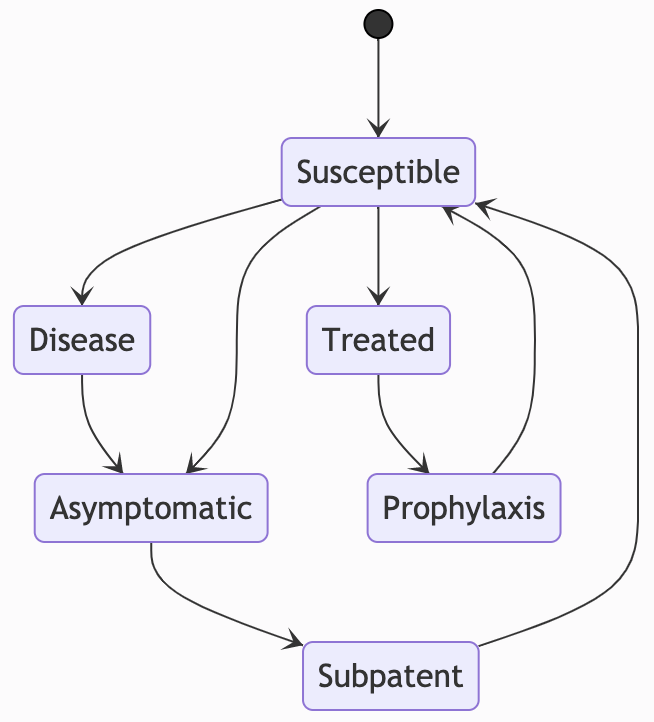
\includegraphics[keepaspectratio=true, scale=0.8]{images/disease-state-transition-diagram.png}
	\caption{Human host disease states transition}
\end{figure}

Models from \gls{swisstph} had at their core individual humans with varying parasite densities. The varying level then will affect the possibilities of the state transition. Infected human will be more likely transit to the next level when they have higher densities.

\subsection{Demography}

\subsubsection{Age}
\improvement{TODO: Of xx papers, xx stratified individuals by age}
Commonly, age was used in the calculation of human biting rates, because of its strong correlation with body surface area.
Other age-varying factors were adaptive and maternal immunity and duration of infection.
\gls{pfpr} was usually calculated at age groups.
If intervention were targeting specific age group, for example \gls{rts}, stratification in model output was used to assess the impact at different age groups.


Human population data
Often lack in some areas
Could be estimated through satellite observations
Paper high resolution population maps for low income nations: combining land cover and census in East Africa

\subsubsection{Birth and Death}
Birth and death was simulated in some \gls{abm} models.
Birth was carefully calculated to ensure a constant population in \improvement{TODO: add citation}.
However in south Saharan African countries, the stalled decreasing trend of malaria cases may related to the increasing population.

An universal death rate was introduced to some models \improvement{TODO: add citations} to ensure a constant age distribution. Death rate was also calculated based on the severity of malaria infection.

\subsubsection{In and Out}
Increasing human mobility is creating highly favorable conditions for the persistence of diseases being targeted for elimination.
Host mobility is not a top priority factor for the malaria model.
In malaria elimination scenario, imported cases is an most important threat.
Modeling population flow in that case would be helpful for countries in elimination stage to quantify the threats.
In that case, predictive models of human movement are needed to help inform how best to target strategies.

One study focused to fit trip data to the gravity model and radiation model\cite{Marshall2018}.
The relationships between travel distance and frequency was studied.
Other model\cite{acevedo_spatial_2015} used extend Ross-Ronald model to the interplay between spatial transmission heterogeneity and human mobility, and their combined influence on prevalence and \gls{R0}.
These models may help predict the spatial transmission of malaria parasites and inform strategies to control their spread.

On the contrast to host mobility, vector mobility is rarely included in the mathematical models.

\subsection{Immunity}

The immunity was separated into several categories:

\paragraph{Maternal Immunity}%
\label{par:maternal_immunity}
Maternal immunity, acquired from mother. Children will get the maternal antigen from mother. Their immunity level were inherited from their mother's level. The maternal immunity will protect new born infant from infections, and will decay after 6 months.

\paragraph{acquired immunity}%
\label{par:acquired_immunity}
Acquired immunity.`\ ' including clinical immunity and \improvement{add another type}.
Acquired immunity alters the likelihood that infection results in clinical disease, modifies onward infectivity to mosquitoes, affects the detectability of infection, and modifies the duration of parasitaemia.

Specific antibodies against \textit{Plasmodium} decay over time.
\improvement{TODO: among xx studied paper, xx dictated the rate of decay of immunity level}
Different versions of models describe the rate of immunity decay differently.

\improvement{TODO: Describe the decay rate mathematically}

\section{Vector}%
\label{sec:vector}
Models most commonly assessed the interventions impacting vector mortality, such \gls{irs}, \gls{itn} and larval source management.
Detailed implementation of vector life cycle and entomology were common.
Mosquito behaviors, such as lifespan, density-dependent larval development, feeding and resting behavior, feeding habits, movement patterns and biting frequency, often modeled in detail.
When models also included a spatial component, malaria transmission generally required vector and host to be co-located.

\subsection{Entomology}
Simulations used a ‘decision tree’ to represent the timing of movements and other necessary actions.
The gonotrophic cycle of a female mosquito begins with a blood meal taken from a host.
The mosquito will rest and wait for digestion.
It may take several blood meals before searching for a breeding site for oviposition.
After egg maturation, the mosquito tries to find a suitable site and then lay 80 – 100 eggs.
Then mosquitoes will search for another blood meal and repeat the gonotrophic cycle.
Larvae emerge from eggs.
After four morphologically larval instars, larvae transform into pupae which develop into adult mosquitoes.
The duration of the larval period depends mainly on temperature, lasts 7-15 days in tropical areas.

\subsection{Adult Mosquitoes}

\subsubsection{Species}
\textit{An. gambiae} is the dominated species used in most models.
However different species, including \textit{An. arabiensis}, \textit{An. vagus}, \textit{An. stephensi}, \textit{An. darlingi}, were also included in some other models.
Different combinations of species were also common in the implementation.
The host preferential and feeding habits of different species are the most important factors affect the intervention effectiveness.
Generally, the lower proportion of human blood feeding and night blood feeding, the lower the efficiency of the intervention targeted at protection in night, such as \gls{llins}.

\subsubsection{Endophily}
Research papers often take endophily as a fixed parameter in the model, which means for each different vector there is one according level of endophily.

And the model used in the research often use a

Does endophily change over time or based on the seasons? Often in the cold weather, some vector species tend to reside in the indoor environment. Not covered in the papers.

\improvement{Create a database from research papers to see the different settings of endophily of vector species}

\paragraph{Daily survival rate}

\paragraph{Human visiting rate}

\paragraph{Extrinsic Incubation Period}
Average incubation period in days
Extrinsic incubation period
Features describing a group of vectors (may influenced by interventions)
The composition of the species of given an area
The distribution of vectors
The overall birth rates of vectors
Types of birth rates defined in the papers
fixed (constant)
The distribution of the length of feeding cycle
Related to species, interventions used
\improvement{add two figures(using normal distribution)}
Distribution before intervention
Distribution after intervention

The distribution of the life span of a given group

\paragraph{Cycling Repeating Rate}
Cycling repeating rate

\paragraph{Flying ability}
How long could it fly in a given time

Mathematical function:

A spatial distribution for a given time, e.g.

The ability could determine whether an infectious bite could be transmitted from one to another in a long distance.

\improvement{TODO:
	Add distribution example
	Add mathematical function
	Collect information from papers and create a database}
\paragraph{HBI}
\gls{hbi}
Related to species, intervention
Usage of \gls{llins} and/or \gls{irs} will discourage human biting divert more bites onto non-human hosts

The birth rates may vary in the different settings.
E.g. `\ ' for a colony of germ in the, the reproduction process follows to a logistic growth:
\improvement{TODO: added an example figure of logistic growth}

Does the birth rate of vectors follow the same line?

\subsection{Larval}

Larvae feeds on yeasts, bacteria and organic matters.
After four moults, larvae become pupae, and then develop into adult mosquitoes.

\paragraph{Carrying capacity}%
\label{par:carrying_capacity}
\begin{parameter}
	Carrying capacity, describe how many mosquito larvae or pupae an environment can support.
\end{parameter}

\paragraph{competition}%
\label{par:competition}
Two different forms of density-dependent competition in the larval stages:

\begin{itemize}
	\item contest competition: number of larvae reaches a limit as initial edge density increases. Due to (i) increased mortality at higher density (ii) increased developmental time (iii) reduced larval size.
	\item scramble competition: number of larvae decreases at higher initial egg density. Due to (i) cannibalism of early instar larvae by late instar and (ii)increased population of predators.
\end{itemize}

Environmental larval source management -- reduce carrying capacity

IRS or LLINs - reduction in oviposition -- reduce density-dependent competition between larvae -- decreased larval mortality

\paragraph{Larval Population Dynamics}%
\label{par:larval_population_dynamics}

\begin{parameter}
	\label{para:eggs_laid_per_day}

	Eggs Rate: $\beta$, number of eggs laid per day by each female mosquito.
	\[
		\beta=\frac{eggs\:laid\:in\:life\:time}{expected\:life\:time}
		.\]

\end{parameter}

\subsection{Vector Resistance Against Chemicals}

Discriminating dose bioassays (WHO tube assay, WHO cone assay, CDC bottle assay) are a practical option for control programmes to assess the proportion of the mosquito population that are killed by a standard dose.
Although the simple bioassay has its limitations, it provides a useful measure to link the severity of mosquito insecticide resistance estimated in the field to the results of experimental hut trials evaluating new products.

Strong association between the level of resistance and mosquito mortality observed in the experimental hut trial\cite{Sherrard-Smith2018b}.
\unsure{to understand how they made the connection: did the researcher match the bioassay result to the experimental hut trial data? Find conclusions and methods in the paper and summarized it in this document.}
\unsure{how does mosquito resistance affect the repel rate? Why do the mosquitoes don't like the pyrethroid  smell? And why does the mosquitoes' repel rate drops down when the resistance level goes up?}

Resistance level in discriminating bioassay: the percentage of mosquitoes surviving 24-hours following exposure.

The impact of reduced susceptibility of mosquito:
\begin{itemize}
	\item the initial efficacy is reduced
	\item the active life-length of the insecticide is shorter as fewer mosquitoes are susceptible
\end{itemize}

\change{add the mathematical equation that describe the decrease.}

One comment on the second point is that it seems there are some certain level of threshold for the resistance level and active ingredient. When combining these two factors, we might able to calculate the overall efficacy of the effective length.

\subsection{Measurement of Resistance}

Bioassay:

\begin{itemize}
	\item Discriminating Bioassay
	\item Intensity Bioassay
	\item Mechanism Bioassay
	\item Non-standard Bioassay
\end{itemize}

\section{Interventions}

Interventions could broadly be divided into those targeted at the human host (e.g. pharmacological) or the vector.

Two core interventions defined by WHO: \gls{llins}, \gls{irs}

Effects of \gls{llins} and \gls{irs}:

\begin{itemize}
	\item Deferred from entering, measured by by the number of mosquitoes caught in a hut with an intervention compared to a control hut
	\item enter the hut and either exit without feeding
	\item Die
	\item Successfully blood-fed
	\item Lower down the survival rates for adults mosquitoes in \gls{eip}
	\item less eggs being oviposited in breeding sites
\end{itemize}

Effects of \gls{irs} \cite{Sherrard-Smith2018b}:

\gls{irs} product effectiveness varies depending on factors including:

\begin{itemize}
	\item impact on mosquito populations (for example, an ability to kill or deter mosquitoes from entering a sprayed structure);
	\item impact duration (the residual half-life);
	\item where and when sprays are deployed (local malaria endemicity, seasonality of transmission and timing of IRS, mosquito species, human behaviour and net-use), and;
	\item spray quality and coverage.
\end{itemize}

Realistic intervention variables, including attrition of LLINs due to wear and tear, waning of insecticides used within IRS or LLINs, and prespecified correlation between interventions and rounds of the same intervention was included in some models\cite{Walker2016}.

Interventions targeting adult mosquitoes have the benefit of reducing the probability that an infected mosquito survives sporogony to become infectious, but reduced oviposition will lower the inner competition of larvae, hence reduce the mortality of larvae.
While, interventions targeting larvae will result in a drop in mosquito density, but the proportion of infected mosquitoes will remain the same, or even increase(due to the reduced competition in adult mosquitoes for blood meals)

\subsection{effectiveness}
\improvement{TODO: what kind of index studies focused? EIR? DALYs? Prevalence?}
Studies focused on the assessment of the impact of interventions on malaria transmission, mosquito prevalence, \gls{eir}, cases averted.

Prevalence results from Uganda \gls{rct}\cite{Staedke2020}:
\begin{center}
	\begin{tabular}{c c c c}
		Type        & 6 months & 12 months & 18 months \\
		\hline
		\gls{llins} & 15       & 13        & 14        \\
		\gls{pbo}   & 11       & 11        & 12        \\
	\end{tabular}
\end{center}

\subsection{attrition}
From Tanzania\cite{Protopopoff2018} \gls{rct}, the permethrin and \gls{pbo} concentration dropped at a steady rate for both standard \gls{llins} and Pyrethroid-PBO \gls{llins}:

\begin{center}
	\begin{tabular}{cccc}
		\toprule
		chemical             & 0 months & 12 months & 21 months \\
		\midrule
		Permethrin (Regular) & 21.4     & 21.5      & 16.7      \\
		Permethrin (PBO)     & 20.9     & 14.7      & 12.2      \\
		PBO                  & 9.5      & 2.9       & 1.6       \\
		\bottomrule
	\end{tabular}
\end{center}

From Uganda\cite{Staedke2020}, the \gls{pbo} dropped:
\begin{center}
	\begin{tabular}{c c c}
		\toprule
		chemical     & 0 months & 12 months \\
		\midrule
		PermaNet 3.0 & 26.18    & 15.28     \\
		Olyset Plus  & 8.17     & 5.04      \\
		\bottomrule
	\end{tabular}
\end{center}

Usage attrition from Tanzania\cite{Protopopoff2018}:

\begin{center}
	\begin{tabular}{c c c}
		\toprule
		index     & 4 months & 21 months \\
		\midrule
		ownership & 97.6     &           \\
		access    & 89.6     & 70.2      \\
		usage     & 76.9     & 50.6      \\
		\bottomrule
	\end{tabular}
\end{center}

\begin{center}
	\begin{tabular}{c c c c}
		\gls{irs}      & 0 months & 9 months & 12 months \\
		Actellic 300CS & 0.99     & 0.82     & 0.59      \\
	\end{tabular}
\end{center}

Usage attrition from Uganda\cite{Staedke2020} showed a much slower trend in the decease in usage:

\begin{center}
	\begin{tabular}{c c c c}
		index             & 6 months & 12 months & 18 months \\
		ownership         & 97       & 95        & 91        \\
		adequate coverage & 71       & 63        & 51        \\
		usage             & 85       & 79        & 73
	\end{tabular}
\end{center}

\subsection{PBO}

\[
	PBO = 3.41 + 5.88 \frac{((1-\beta) - 0.5)}{1 + 0.78 ((1-\beta) - 0.5)}
	.\]
\[
	\gamma_a = \frac{e^{PBO}}{1 + e^{PBO}}
	.\]
\[
	\gamma_a = 1 - \beta
	.\]
\[
	\gamma_h' = 0.63 + 3.997 ( \gamma_a - 0.5 )
	.\]
\[
	\gamma_h = \frac{e_{\gamma_h'}}{1+e^{\gamma_h'}}
	.\]

\subsection{IRS}
Four insecticide gradients, pyrethroids (including deltamethrin, lambda-cyhalothrin and alpha-cypermethrin) are the main insecticides used by \gls{nmcp} for \gls{irs}.

\section{Costs}
Cost of Interventions increases when coverage increase.\cite{Winskill2017a} considered two approaches to simulate the function:
\begin{itemize}
	\item linear increases in cost associated with increasing coverage
	\item delivery cost increases logarithmically with increasing coverage
\end{itemize}

Total cost was assumed to consist of two components: the commodity and the delivery. The commodity part of cost follows U-shape curves follows the marginal cost formula.

$$ MC = \frac{\Delta C}{\Delta Q} $$

In the short run, marginal cost ($MC$) drops when quantity($Q$) increases, then increase as $Q$ increases.

The delivery part increase as coverage increase. For the linear assumption, J

\begin{table}[htpb]
	\centering
	\caption{Cost of Malaria Interventions}
	\label{tab:cost_of_malaria_interventions}
	{\small
		\begin{tabular}{cSSSSSSSS}
			\toprule
			Studies           & {year} & {distributing \gls{llins}} & {\gls{irs}(per person per year)} & {three rounds of seasonal Chemoprevention(per child per year) } & {Non-drug cost of mass screen and treatment (per person per round)} & {Non-drug cost of mass drug administration (per person per round) } & {Full course of dihydroartemisin-piperaquine} & {Treatment of uncomplicated malaria with artemether-lumefantrine} \\
			\midrule
			\cite{Walker2016} & 2016   & 7.03                       & 8.80                             & 5.25                                                            & 5.63                                                                & 2.98                                                                & 1.65                                          & 2.50                                                              \\
			\bottomrule
		\end{tabular}
	}
\end{table}

\subsection{\gls{llins}}

\subsection{Costs of IRS}
Range from USDA 2–3 to roughly USDA 20 per unit\cite{Oxborough2016}
(a unit is standardized across products to cover approximately 250 of wall surface)

\section{Environment}%
\label{sec:environment}
Core environmental aspects related to vector activity were included, such as water sources for oviposition, houses for blood meal locations, and meteorological data to account for seasonal patterns in transmission.
Rainfall and temperature data were regularly used.
Seasonality in larval carrying capacity informed by seasonal patterns in rainfall\cite{Walker2016}.

Perennial and seasonal settings were two concepts describing the seasonal feature in sub-Saharan region.

\section{Parameters}

Most models used past literature or simulations to determine baseline parameter values.
Due to the nature of certain inputs, many parameters cannot or have not been estimated in field studies, and consequently authors used expert knowledge to select these values.

Studies used models that were either previously calibrated to data or presented calibration as a component of their work.
Calibration techniques included the use of calibration vectors, least squares, maximum likelihood functions, and visual estimations.
Bayesian techniques for model fitting could provide credible intervals alongside point estimates of parameters.
Calibrating all model parameters to data is not implemented by most researchers, which necessarily excludes certain parameter combinations that could produce accurate calibrations.

Average eggs lay by female \textit{Anopheles}: 80 - 100 eggs.

Duration of the larval period depends on temperature, in tropical areas, lasts 7 - 15 days.\cite{bayoh_lindsay_2003}

Carrying capacity in aquatic stage: describe how many mosquito larvae/pupae an environment can support

\subsection{Experimental Hut Trail}

Experimental hut studies typically report 24-h productinduced: mortality, blood-feeding inhibition, exophily and deterrence.

Outcome:

\begin{parameter}
	\label{eht:mortality}

	Mortality: The number of female mosquitoes found in the hut which are dead on collection or die within the next 24-h
	\[
		Mortality = \frac{D}{N}
		.\]
\end{parameter}


\begin{parameter}
	\label{eht:exophily}

	Exophily: the number of female mosquitoes in exit traps (E) compared to the sum of the number collected in the hut and exit traps (N)
	\[
		Exophily = \frac{E}{N}
		.\]

\end{parameter}

\begin{parameter}
	\label{eht:blood_fed}

	Blood feeding: The number of mosquitoes that are blood fed which were collected in the hut and exit traps
	\[
		BloodFed = \frac{B}{N}
		.\]
\end{parameter}

\begin{parameter}
	\label{eht:Deterrence}

	Deterrence: Reduction in the entry rate of mosquitoes into experimental huts with or without.
	\[
		Deterrency = \frac{N_C - N_T}{N_C}
		.\]
\end{parameter}

Explanatory factors:

\begin{parameter}
	\label{eht:experimental_hut_types}
	Experimental hut types: West or East African design

\end{parameter}

\begin{parameter}
	\label{eht:wall_substrate}
	Wall substrate: Cement or mud

\end{parameter}

\begin{parameter}
	\label{eht:chemical_class_used}
	Chemical types used in \gls{eht}.

	For IRS: carbamate, clothianidin, organophosphate and pyrethroid

	For LLINs:
	\improvement{TODO: list the chemical class used in the LLINs}

\end{parameter}

Prediction of \gls{eht} outcomes using explanatory factors, combining linear algebra and non-linear transformation\cite{Sherrard-Smith2018b}:

\[
	\pi_i = logit^{-1} \frac{\ln \pi_i}{1-\pi_i} = \frac{ \exp( \beta + \sum_h \beta_h X^{hi} ) }{ 1 - \exp( \beta + \sum_h \beta_h X^{hi} ) }
	.\]

$\beta_h X^{hi}$ denotes explanatory factors times covarite, which is the linear transformation of the explanatory hypothetical space. The middle part of the formulation then project $\mathbb{R} \twoheadrightarrow (0,1)$.

\section{Evaluation and Validation}
Validation was performed on some models.
All major model frameworks were reported as validated.
Validation techniques were rarely explained in detail.
When described, validation was most commonly performed by running a calibrated simulation, and comparing model outputs to a dataset not used for calibration.
For example, validation against \gls{rct}, or \gls{eht}.

Methods of comparing models to data were rarely explained; use of a square distance function , log likelihoods and docking techniques were outlined.
Successful model validation was often used to justify extending a model framework to include interventions or to assess their potential impact in the location of interest.
A number of studies concluded that their model did not accurately fit the data used for validation, suggesting incomplete data may explain any discrepancies.

Some studies explicitly mentioned sensitivity analysis or described parameter variation and comparison of outputs.
The techniques used were generally informal, with methods used rarely explained in detail, and reporting of results was uncommon.
Where sensitivity analysis was explained, it involved altering calibrated baseline parameter values by a fixed percentage and assessing changes to outputs.
Formal techniques employed included Latin Hypercube sampling, regression tree analysis, and one-way and probabilistic sensitivity analysis.

\subsection{Comparing to Randomized Control Trails}

\gls{rct} is the gold standard for assessing intervention efficacy and effectiveness in the field.
Results from \gls{rct} were compared to the model predictions by modellers to determine whether parametrisations satisfactorily match the observed red data\cite{Sherrard-Smith2018b}.
Mean, as well as maximum and minimum impact can be generated by models for assessing.
The parameter sets could be fitted to different \gls{eht} and then compare the results from \gls{eht}.

\subsection{Cross Comparing}
\subsection{Predict Future Results}

\section{Method}%
\label{sec:method}
\subsection{Search strategy and selection criteria}
A literature review was performed.
Database searches of Google Scholar were performed.
Terms relating to malaria, mathematical model, epidemiology, demography, agent-based, individual-based, microsimulation models were included. No limits were placed on publication type, language, location, dates or publication status.

\section{results}%
\label{sec:results}
The search yielded 212 abstracts potentially meeting the inclusion criteria.

\begin{table}
	\centering
	\label{tab:overview_of_the_review}
	\begin{tabular}{c S}
		\toprule
		type             & {number} \\
		\midrule
		inclusion        & 212      \\
		full-text review & 50       \\
		\bottomrule
	\end{tabular}
	\caption{Overview of the review}
\end{table}

% appendix
\appendix
\printglossaries
\printnomenclature
\bibliographystyle{unsrt}
\bibliography{library}

\end{document}
